% Synthetic streams. Numbers come from numbers_generated.tex.
% Differences are written "A minus B = value" so the sign is always explicit.

\section{Results}\label{sec:results}

\subsection{Synthetic streams}\label{sec:res-syn}

Each of the five synthetic generators has three era boundaries at which the prompt features and the risk change; within an era the regime is fixed or alternates between two regimes every $50$ to $80$ steps. Table~\ref{tab:synthetic} reports the mean over \nSeeds{} seeds, and Figure~\ref{fig:frontier-syn} plots post-shift violation against sharpness.

\paragraph{The update does the long-run work.}
Static calibration reaches coverage \synStaticCov{} and rolling calibration \synRollingCov{}, below the target of $0.90$. Every method with the online update is within $0.02$ of the target, consistent with Theorem~\ref{thm:longrun} (the bound is $0.018$ to $0.024$ for these streams and is listed for every experiment in Table~\ref{tab:hyper}). Removing the update from PromptShift-CRC lowers its coverage to \synNoUpdCov{} and raises its post-shift violation from \synPSPost{} to \synNoUpdPost{}. Marginal coverage therefore does not separate the weighting schemes, and we compare them on post-shift violation, maximum local violation and sharpness.

\paragraph{PromptShift-CRC against the matched baseline.}
Adaptive CRC with a window equal to PromptShift-CRC's recent window has post-shift violation \synMatchedPost{}, against \synPSPost{} for PromptShift-CRC. Paired by seed (Table~\ref{tab:paired}), PromptShift-CRC minus the matched baseline is between \synPostMatchedLo{} and \synPostMatchedHi{} across the five streams, and PromptShift-CRC is lower in only \synPostMatchedLowerMin{} to \synPostMatchedLowerMax{} of \nSeeds{} seeds, so it is slightly \emph{worse} on local validity. It is sharper: the difference in mean threshold is between \synThrMatchedLo{} and \synThrMatchedHi{}, and PromptShift-CRC is lower in \synThrMatchedLowerMin{} to \synThrMatchedLowerMax{} of \nSeeds{} seeds. The two differences have opposite signs and are of the same size, about half a percentage point, so the comparison is a trade-off and not a win.

\paragraph{What the components do.}
The gate buys validity at a cost in sharpness. PromptShift-CRC minus the variant with no gate has post-shift violation between \synPostNoGateLo{} and \synPostNoGateHi{} (lower in \synPostNoGateLowerMin{} to \synPostNoGateLowerMax{} of \nSeeds{} seeds) and threshold between \synThrNoGateLo{} and \synThrNoGateHi{}. The kernel weights do the opposite. The variant that keeps only the gate and the recency window has post-shift violation \synGateRecPost{} and mean threshold \synGateRecThr{}, against \synPSPost{} and \synPSThr{} for PromptShift-CRC. The kernel weights with the update but without the gate and the recency fallback have the sharpest thresholds among these variants (\synKernelUpdThr{}) and the highest post-shift violation (\synKernelUpdPost{}).

\paragraph{Frontier gap.}
A fairer comparison asks whether a method does better than Adaptive CRC at the same sharpness. Table~\ref{tab:frontier_syn} gives the frontier gap. For PromptShift-CRC it ranges from \PSfrontierSynLo{} to \PSfrontierSynHi{} over the five streams (standard error at most \PSfrontierSynSEmax{}) and is negative on \PSfrontierSynBelowCount{} of the five streams. No stream shows more than about half a percentage point of post-shift violation recovered by the drift-aware components.

\paragraph{Stronger online methods.}
DtACI \citep{gibbs2024online}, which runs several step sizes and weights them online, has post-shift violation \synDtACIPost{} on average, and PromptShift-CRC minus DtACI is between \synPostDtACILo{} and \synPostDtACIHi{} on the five streams, with PromptShift-CRC higher in every stream. Its threshold is also lower. Part of this comes from over-coverage: DtACI's coverage is \synDtACICov{} on average, above the target, which flatters its local violation, and the frontier gap is the fairer view. Quantile tracking is worse than every weighted rule that uses the update on these streams. The density-ratio rule is close to PromptShift-CRC. Among the online methods we tested, the handling of the step size matters about as much as the choice of weights.

\begin{figure}[t]
\centering
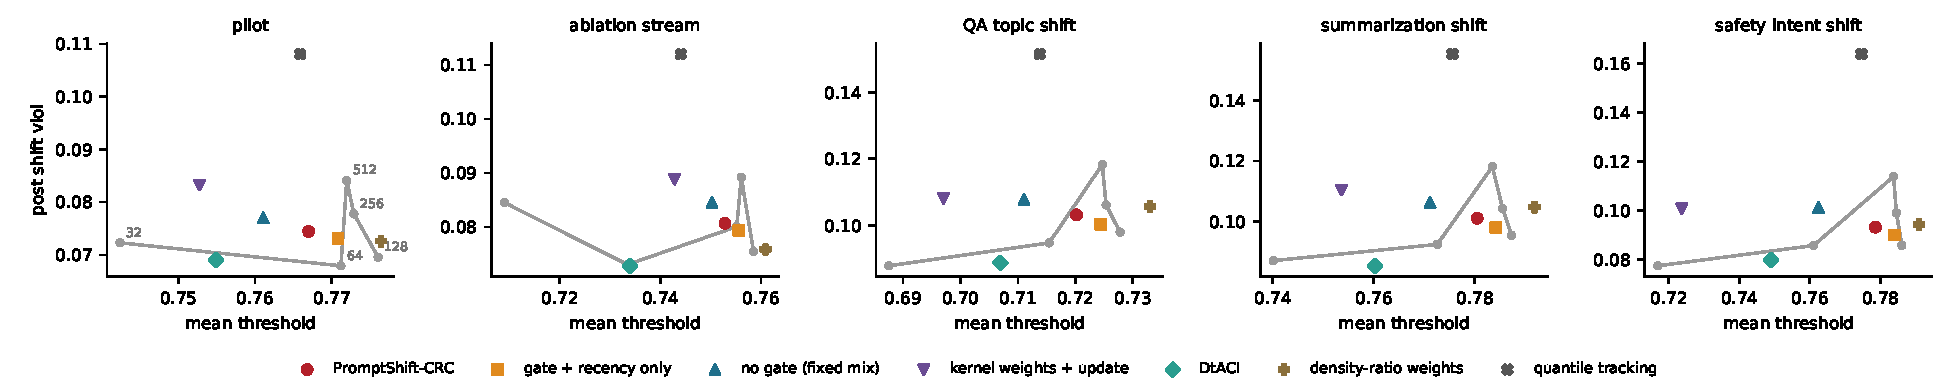
\includegraphics[width=\textwidth]{figures_v2/fig_frontier_synthetic.pdf}
\caption{Validity and sharpness on the five synthetic streams (mean over \nSeeds{} seeds). The grey curve is Adaptive CRC with windows $32$, $64$, $128$, $256$, $512$ (labelled on the first panel); points are other methods. Lower is better on both axes.}
\label{fig:frontier-syn}
\end{figure}
